\chapter{Chamadas de Sistema}
\chapterauthor{Cauã Marques da Silva, Felipe de Castro Duchen Auroux, Felipe de Oliveira Renó, Vicente Pinto Tomás Junior}
%-------------------------------------------------------------------------------
\section{Descrição}
%-------------------------------------------------------------------------------

As chamadas de sistema são o mecanismo pelo qual o sistema operacional fornece aos processos acesso aos recursos do sistema. Essencialmente, as chamadas de sistema são a forma pela qual os processos têm acesso aos arquivos, diretórios, ao relógio, teclado e até mesmo a outros processos.

O sistema operacional oferece esse mecanismo para poder manter a separação entre os dois principais modos de operação do processador: supervisor e usuário. No modo supervisor o processador pode executar qualquer instrução e interagir com outros componentes físicos do sistema; já no modo usuário o processador está restrito a apenas um subconjunto dessas instruções e não pode interagir com outros componentes físicos do sistema. Esse isolamento busca impedir que um processo, defeituoso ou malicioso, assuma controle dos recursos do sistema.

Além disso, a interface criada por esse mecanismo oferece aos programas uma abstração dos recursos do sistema, ou seja, um programa não precisa conhecer o hardware responsável pela memória se ele deseja salvar um arquivo, basta que ele peça ao sistema operacional. Ademais, o programa não precisa nem saber como a informação será efetivamente salva na memória, ele apenas precisa fornecer o que deseja salvar e o sistema operacional lidará com o resto.

%-------------------------------------------------------------------------------
\section{Decisões de Arquitetura e Design}
%-------------------------------------------------------------------------------

As chamadas de sistema estão diretamente ligadas à forma como o núcleo é estruturado; na literatura discutem-se, principalmente, duas arquiteturas: núcleo monolítico e micronúcleo.

A arquitetura monolítica, essencialmente, se baseia em concentrar as operações de nível de sistema dentro do núcleo, ou seja, a gerência de memória, o sistema de arquivos, as pilhas dos protocolos de rede e outros existem no espaço do núcleo (são executados em modo supervisor).

Na arquitetura micronúcleo as operações de nível de sistema são transferidas para o espaço do usuário (são executadas em modo usuário) por módulos próprios separados do núcleo. O núcleo fica, portanto, responsável por escalonar e gerenciar a comunicação entre os processos que agora, também, incluem os módulos do sistema.

Dessa forma, as chamadas de sistema em um núcleo monolítico são executadas em modo supervisor e interagem diretamente com os recursos do sistema; em um micronúcleo, as chamadas seriam transformadas em trocas de mensagens entre o processo fazendo a chamada e o processo responsável pelo recurso do sistema, de forma que o micronúcleo funcionaria apenas como um mediador encaminhando essas mensagens. A Figura \ref{fig:arquiteturas-nucleo} ilustra as principais diferenças entre as duas abordagens.

\begin{figure}[htbp]
    \centering
    \resizebox{\textwidth}{!}{%
    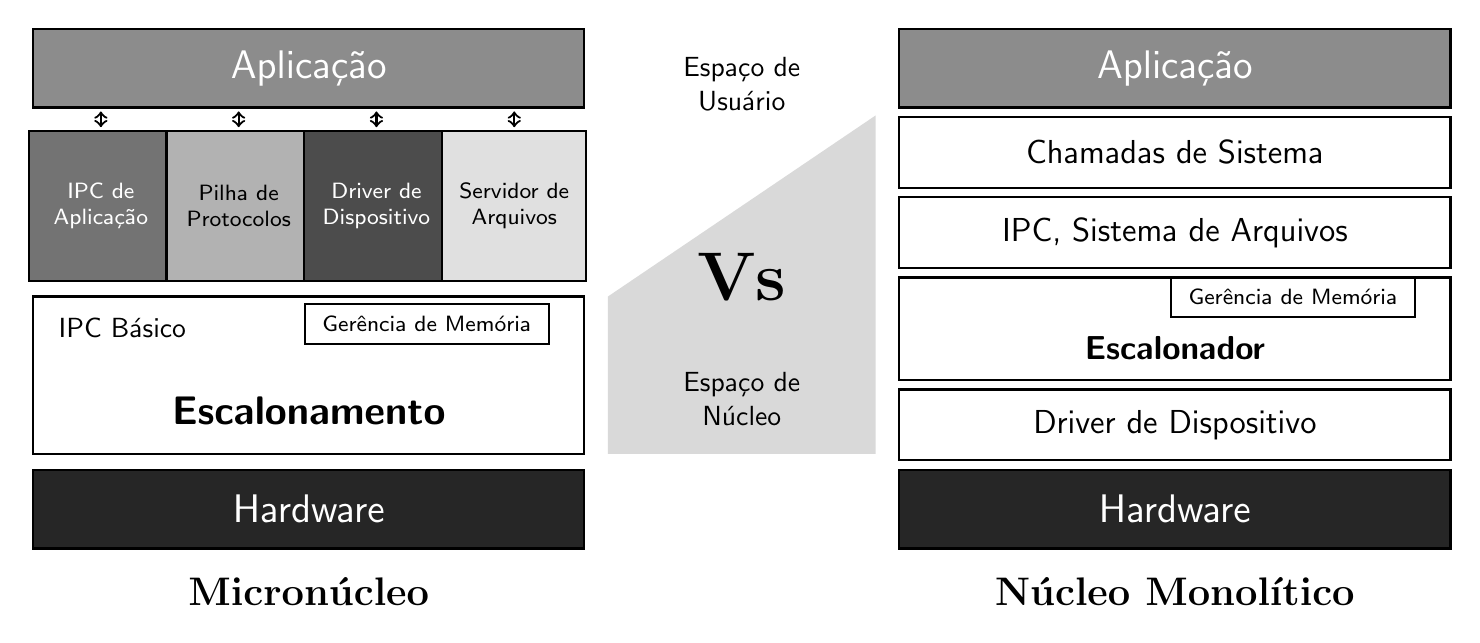
\begin{tikzpicture}[
        font=\sffamily,
        layer/.style={draw=black, thick, minimum height=1cm, align=center, inner sep=4pt},
    ]

    %====================== MICRONÚCLEO (esquerda) — topo em y=6.6 ======================
    \node[layer, fill=black!85, text=white, minimum width=7cm] (mk-hw) at (3.5, 0.5) {\Large Hardware};

    \node[layer, fill=white, minimum width=7cm, minimum height=2.0cm] (mk-kernel) at (3.5, 2.2) {};
    \node[font=\sffamily, anchor=north west] at (0.2, 3.05) {IPC Básico};
    \node[layer, fill=white, minimum width=3.1cm, minimum height=0.5cm] (mk-mm) at (5.0, 2.85) {\footnotesize Gerência de Memória};
    \node[font=\sffamily\bfseries\Large] at (3.5, 1.75) {Escalonamento};

    \node[layer, fill=black!55, text=white, minimum width=1.72cm, minimum height=1.9cm, text width=1.55cm, font=\sffamily\footnotesize] (mk-ipc)   at (0.86, 4.35) {IPC de Aplicação};
    \node[layer, fill=black!30, minimum width=1.72cm, minimum height=1.9cm, text width=1.55cm, font=\sffamily\footnotesize]             (mk-proto) at (2.61, 4.35) {Pilha de Protocolos};
    \node[layer, fill=black!70, text=white, minimum width=1.72cm, minimum height=1.9cm, text width=1.55cm, font=\sffamily\footnotesize] (mk-drv)   at (4.36, 4.35) {Driver de Dispositivo};
    \node[layer, fill=black!12, minimum width=1.72cm, minimum height=1.9cm, text width=1.55cm, font=\sffamily\footnotesize]             (mk-fs)    at (6.11, 4.35) {Servidor de Arquivos};

    \node[layer, fill=black!45, text=white, minimum width=7cm] (mk-app) at (3.5, 6.1) {\Large Aplicação};

    \foreach \x in {0.86, 2.61, 4.36, 6.11} {
        \draw[<->, thick] (\x, 5.35) -- (\x, 5.55);
    }

    \node[align=center, font=\bfseries\Large] at (3.5, -0.55) {Micronúcleo};

    %====================== SEPARADOR VS ======================
    \fill[black!15] (7.3,1.2) -- (10.7,1.2) -- (10.7,5.5) -- (7.3,3.2) -- cycle;
    \node[font=\bfseries\Huge] at (9.0, 3.45) {Vs};
    \node[font=\sffamily, align=center] at (9.0, 5.9) {Espaço de\\Usuário};
    \node[font=\sffamily, align=center] at (9.0, 1.9) {Espaço de\\Núcleo};

    %====================== NÚCLEO MONOLÍTICO (direita) — topo em y=6.6 ======================
    \node[layer, fill=black!85, text=white, minimum width=7cm] (mono-hw) at (14.5, 0.5) {\Large Hardware};

    \node[layer, fill=white, minimum width=7cm, minimum height=0.9cm] (mono-drv) at (14.5, 1.57) {\large Driver de Dispositivo};

    \node[layer, fill=white, minimum width=7cm, minimum height=1.3cm] (mono-sched) at (14.5, 2.79) {};
    \node[layer, fill=white, minimum width=3.1cm, minimum height=0.5cm] (mono-mm) at (16.0, 3.19) {\footnotesize Gerência de Memória};
    \node[font=\sffamily\bfseries\large] at (14.5, 2.55) {Escalonador};

    \node[layer, fill=white, minimum width=7cm, minimum height=0.9cm] (mono-ipc) at (14.5, 4.01) {\large IPC, Sistema de Arquivos};

    \node[layer, fill=white, minimum width=7cm, minimum height=0.9cm] (mono-sc) at (14.5, 5.03) {\large Chamadas de Sistema};

    \node[layer, fill=black!45, text=white, minimum width=7cm] (mono-app) at (14.5, 6.1) {\Large Aplicação};

    \node[align=center, font=\bfseries\Large] at (14.5, -0.55) {Núcleo Monolítico};

    \end{tikzpicture}%
    }
    \caption{Comparação entre as arquiteturas de micronúcleo e núcleo monolítico.}
    \label{fig:arquiteturas-nucleo}
\end{figure}

Nesse contexto, para o desenvolvimento das chamadas de sistema neste projeto, adotou-se uma abordagem de núcleo monolítico visando simplificar os detalhes de implementação das chamadas em si, uma vez que as mesmas podem interagir diretamente com os recursos do sistema. Consequentemente, essa abordagem acarreta em um núcleo mais complexo (no que se refere à quantidade de partes e responsabilidades do núcleo), o que reduz a modularidade e introduz mais pontos de falha no sistema (uma vez que as chamadas de sistema acontecem em modo supervisor, o que pode ser perigoso caso haja falhas no código).

%-------------------------------------------------------------------------------
\section{Detalhes da Implementação}
%-------------------------------------------------------------------------------

Há quatro principais componentes envolvidos em realizar uma chamada de sistema, sendo eles: o invocador, o tratador SVC, o tratador de chamada de sistema e a tabela de chamadas de sistema. A Figura \ref{fig:syscall-flow} ilustra o fluxo de execução entre esses quatro componentes, detalhado nos parágrafos a seguir.

\begin{figure}[htbp]
    \centering
    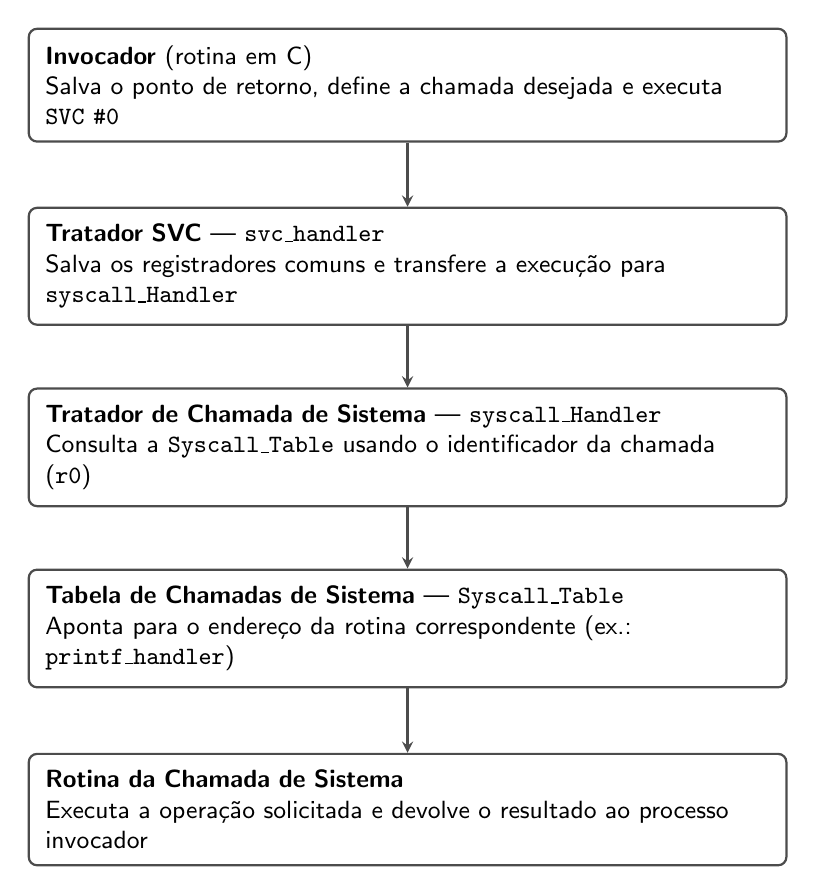
\begin{tikzpicture}[
        >=stealth,
        box/.style={
            rectangle,
            draw=black!70,
            thick,
            rounded corners=3pt,
            text width=9.2cm,
            align=left,
            fill=white,
            font=\small\sffamily,
            inner sep=6pt
        },
        arrow/.style={->, thick, draw=black!70}
    ]

    \node[box] (b1) at (0, 0)     {\textbf{Invocador} (rotina em C)\\Salva o ponto de retorno, define a chamada desejada e executa \texttt{SVC \#0}};
    \node[box] (b2) at (0, -2.3)  {\textbf{Tratador SVC} --- \texttt{svc\_handler}\\Salva os registradores comuns e transfere a execução para \texttt{syscall\_Handler}};
    \node[box] (b3) at (0, -4.6)  {\textbf{Tratador de Chamada de Sistema} --- \texttt{syscall\_Handler}\\Consulta a \texttt{Syscall\_Table} usando o identificador da chamada (\texttt{r0})};
    \node[box] (b4) at (0, -6.9)  {\textbf{Tabela de Chamadas de Sistema} --- \texttt{Syscall\_Table}\\Aponta para o endereço da rotina correspondente (ex.: \texttt{printf\_handler})};
    \node[box] (b5) at (0, -9.2)  {\textbf{Rotina da Chamada de Sistema}\\Executa a operação solicitada e devolve o resultado ao processo invocador};

    \draw[arrow] (b1) -- (b2);
    \draw[arrow] (b2) -- (b3);
    \draw[arrow] (b3) -- (b4);
    \draw[arrow] (b4) -- (b5);

    \end{tikzpicture}
    \caption{Fluxo de execução de uma chamada de sistema, através dos quatro componentes envolvidos.}
    \label{fig:syscall-flow}
\end{figure}

Os invocadores são as rotinas encapsuladas pelas funções em C que oferecem as chamadas de sistema para os processos. Essas precisam registrar o ponto atual da execução (para que se possa retornar a esse ponto posteriormente), registrar o endereço da rotina que será executada e, então, gerar uma exceção forçando a transferência da execução para o sistema operacional em modo supervisor, como no exemplo do Código \ref{lst:invocador}.

\begin{lstlisting}[language=C, caption={Exemplo de invocador}, label={lst:invocador}]
exemplo:
    push {lr}
    mov r0, #CHAMADA
    SVC #0 
    pop {pc}
\end{lstlisting}

Quando a instrução SVC é usada, o processador gera uma exceção; ele então consulta a tabela de exceções e transfere a execução para a rotina identificada na tabela. O tratador SVC, simplesmente, salva os registradores comuns e transfere a execução para o tratador de chamada de sistemas (Código \ref{lst:svc-handler}).

\begin{lstlisting}[language=C, caption={Tratador SVC}, label={lst:svc-handler}]
svc_handler:
    STMFD sp!, {r1-r12, lr}
    bl syscall_Handler
    LDMFD sp!, {r1-r12, pc}^
\end{lstlisting}

O tratador de chamadas de sistema interpretará pelos argumentos da chamada qual é a intenção do processo e fará uma consulta na tabela de chamadas de sistema (Código \ref{lst:syscall-handler}).

\begin{lstlisting}[language=C, caption={Tratador de chamada de sistema}, label={lst:syscall-handler}]
syscall_Handler:
    ldr r3, =Syscall_Table
    ldr r3, [r3,r0,LSL #2]
    bx r3
\end{lstlisting}

Se possível, ele executará a rotina associada ao endereço na tabela (Código \ref{lst:syscall-table}) e devolverá o resultado e a execução para o processo que fez a chamada de sistema.

\begin{lstlisting}[language=C, caption={Tabela dos endereços das chamadas de sistema}, label={lst:syscall-table}]
Syscall_Table:
    .word printf_handler
    .word abort_handler
\end{lstlisting}

\begin{lstlisting}[language=C, caption={Exemplo de rotina que será de fato executada}, label={lst:printf-handler}]
printf_handler:
    mov r0,r1
    push {lr}
    bl serial_puts
    mov r0, #10
    pop {pc}
\end{lstlisting}


%-------------------------------------------------------------------------------
\section{Interface Pública (API)}
%-------------------------------------------------------------------------------

O subsistema de chamadas de sistema disponibiliza, por ora, duas chamadas, descritas na Tabela \ref{tab:api-syscalls}.

\begin{table}[htbp]
    \centering
    \renewcommand{\arraystretch}{1.3}
    \newcolumntype{Y}{>{\raggedright\arraybackslash}X}
    \begin{tabularx}{\textwidth}{@{}l >{\hsize=0.85\hsize}Y >{\hsize=0.75\hsize}Y >{\hsize=1.4\hsize}Y@{}}
        \hline
        \textbf{Função} & \textbf{Parâmetros} & \textbf{Retorno} & \textbf{Descrição} \\
        \hline
        \texttt{printf} & Ponteiro de \texttt{char} para o texto a ser impresso & \texttt{0} (sucesso)\newline\texttt{-1} (falha) & Imprime o texto passado como parâmetro na saída serial. \\
        \texttt{abort} & --- & \texttt{0} (sucesso)\newline\texttt{-1} (falha)$^{*}$ & Força o reinício da CPU. Em processadores ARM é necessário interagir com o PSCI (\textit{Power State Coordination Interface}). \\
        \hline
    \end{tabularx}
    \caption{Chamadas de sistema disponíveis na API pública.}
    \label{tab:api-syscalls}
\end{table}

{\footnotesize $^{*}$Observação: por enquanto a chamada \texttt{abort} não possui uma forma de retornar nenhum valor, uma vez que o reinício é instantâneo.}
%-------------------------------------------------------------------------------
\section{Testes e Verificação}
%-------------------------------------------------------------------------------

As rotinas que invocam as chamadas de sistema estão encapsuladas em C, então os testes consistiram em invocá-las, verificar, pelo depurador, as alterações no fluxo de execução e observar o resultado da execução das rotinas. A Tabela \ref{tab:testes-syscalls} resume os resultados obtidos.

\begin{table}[htbp]
    \centering
    \small
    \renewcommand{\arraystretch}{1.3}
    \begin{tabular}{@{}p{1.7cm}p{4.6cm}p{4.6cm}@{}}
        \hline
        \textbf{Chamada} & \textbf{Comportamento Esperado} & \textbf{Comportamento Obtido} \\
        \hline
        \texttt{printf} & Mensagem ``Testando alterações'' exibida na tela & Mensagem ``Testando alterações'' exibida na tela \\
        \texttt{abort} & Reinício da CPU, com a mensagem ``Executando em modo ARM bare-metal no QEMU.'' exibida na tela & Salto do endereço corrente para o endereço \textit{start} (sinalizando o reinício), seguido da exibição da mensagem ``Executando em modo ARM bare-metal no QEMU.'' \\
        \hline
    \end{tabular}
    \caption{Resultados dos testes das chamadas de sistema.}
    \label{tab:testes-syscalls}
\end{table}

Essas chamadas de sistema apenas encapsulam rotinas que já existiam (no caso do \texttt{printf}) ou instruções especiais da CPU (no caso do \texttt{abort}); portanto, os casos de borda se restringiram ao que acontece durante uma chamada de sistema, ou seja, se os registradores estavam sendo manipulados corretamente (salvos e depois restaurados), o que foi constatado pela inspeção durante a depuração de ambas as chamadas.